
% ==================================================
%	Aufbau
% ==================================================

\section{Aufbau}
	Eine Skizze des Versuchsaufbaus ist in Abbildung \ref{fig:Aufbau} zu
	\begin{figure}
      \centering
		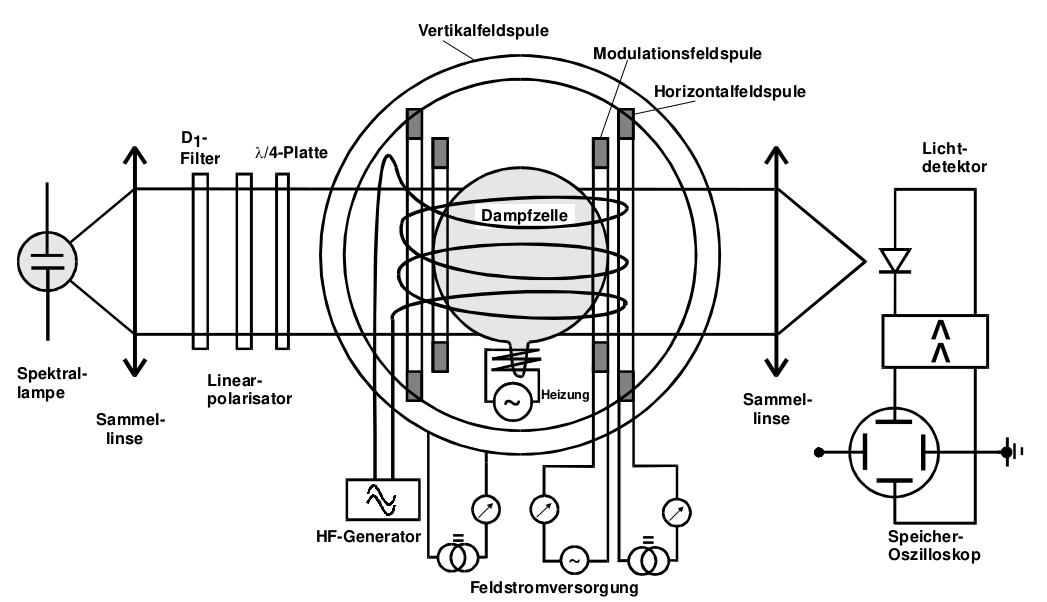
\includegraphics[scale=0.3]{bilder/aufbau}
		\caption{Schematische Abbildung des Versuchsaufbaus.
		\cite{Praktikum}}
		\label{fig:Aufbau}
	\end{figure}
	sehen. Der Aufbau aus Rb-Spektrallampe, Sammellinse und $D_1$ Filter
	erzeugt Licht der Wellenlänge
	$\lambda = \SI{794.8}{\nano\meter}$, welches genau dem $D_1$
	 Übergang
	des Rb-Spektrums ($S_\nicefrac12$ nach $P_\nicefrac12$) entspricht.
	Durch den linear Polarisator und die anschließende $\lambda/4$
	Platte kann zirkular polarisiertes Licht erzeugt werden. Dieses
	tritt durch das Rubidium-Gasgemisch und fällt durch eine
	weitere Sammellinse auf einen Photodetektor, mit dem die einfallende
	Lichtintensität gemessen werden kann. Das Gasgemisch wird dabei auf
	$\SI{50}{\celsius}$ geheizt, um einen optimalen Gasdruck zu
	erreichen. Das Gasgemisch besteht aus \ce{^85Rb} und \ce{^87Rb} Atomen in
	einem unbekannten Verhältnis, sodass zwei Resonanzmagnetfelder  
	mit unterschiedlich stark ausgeprägten Transmittivitätseinbrüchen 
	erwartet werden. 
	Die Apparatur wird so aufgebaut, dass die optische Achse auf der 
	Nord-Süd Achse des Erdmagnetfeldes steht, sodass das Erdmagnetfeld keine 
	dazu senkrechte 
	horizontale Komponente besitzt. Dadurch vereinfacht sich die Korrektur 
	der Messergebnisse um den Einfluss des Erdmagnetfeldes erheblich.

	Die Dampfzelle ist von drei Helmholtzspulen und einer RF-Spule  
	umgeben.
	Die Vertikalfeldspule gleicht das Erdmagnetfeld in 
			vertikaler Richtung aus Windungszahl und Radius sind  
			$N_\text{V}=20$ und $R_\text{V}=11.735$.
		Die Horizontalfeldspule erzeugt ein horizontales 
			Magnetfeld entlang der optischen Achse, Windungszahl und Radius 
			sind 
			$N_\text{H}= 154$ und $R_\text{H}=15.79$.
		Die Sweep-Spule erzeugt ebenfalls ein horizontales 
			Magnetfeld entlang der optischen Achse. Sie sorgt dafür, dass 
			das durch die 
			Horizontalfeldspule erzeugte Magnetfeld um kleine 
			Beträge erhöht werden kann. Windungszahl 
			und Radius sind
			$N_\text{S}=11$ und $R_\text{S}=16.39$.
		Die RF-Spule liegt an der Dampfzelle. An ihr 
			wird die Frequenz $\nu$ für die induzierte Emission 
			eingestellt. Da hier nur die Frequenz entscheidend ist, 
			sind Radius und Windungszahl unerheblich.
	\end{itemize}
	Über ein Potentiometer wird der Spulenstrom von Sweep- und 
	Vertikalfeldspule mit $\SI{0.1}{\ampere}$ pro Umdrehung und bei 
	der Horizontalfeldspule mit $\SI{0.3}{\ampere}$ pro Umdrehung 
	eingestellt. 
	
	Die RF-Spule wird an einen Frequenzgenerator im Bereich 
	$\SI{100-1000}{\kilo\hertz}$ angeschlossen. Auf einem Oszilloskop 
	werden im XY-Modus die Lichtintensität an der Photodiode (Y) gegen 
	die Sweep-Feldstärke (X) dargestellt.
